\chapter{Plataformas}
\label{chap:Plataformas}

Para a localização com os resíduos de comunicação \emph{WiFi} são necessários
sensores que possam capturar estes resíduos e processar qualquer informação
capturada pelo sensor deste trabalho. Esta plataforma de sensor pode ser construída com
qualquer plataforma computacional capaz de ser programada com comunicação
\emph{WiFi}, porém o \emph{hardware} de \emph{WiFi} e seu \emph{software}
controlador deve permitir o Modo Promíscuo.

Este Modo Promíscuo (\emph{promiscuous mode}) é definindo pela capacidade de uma
Placa Adaptadora de Rede \emph{WiFi} (\emph{Network Interface Card} -
\emph{NIC}) receber e interpretar todos os pacotes que trafegam em uma rede ou
em todas as redes que estão em seu alcance, independentemente do destinatário do
pacote. Em seu fucionamento normal, uma \emph{NIC} descarta todos os pacotes que
não são destinados para ela o mais cedo possível, evitando reprocessamento de
dados indesejáveis, por este motivo não são todas as \emph{NICs} que permitem o
Modo Promíscuo. Essa funcionalidade elimina a necessidade de \emph{hardware} ou
\emph{software} em cada um dos dispositivos rastreados.

Neste sentido, elegeu-se duas plataformas de notável importância no mercado atual
e notável facilidade de acesso para qualquer interessado na área. As plataformas
testadas foram o microcomputador \emph{Raspberry Pi} e o microcontrolador
\emph{ESP8266}. Ambos  foram escolhidos pelo domínio do segmento de Prototipação
e Faça Você Mesmo  (\emph{Do It Yourself} - \emph{DIY}) dentro do campo de IoT.
Outro líder de segmento, o \emph{Arduino}  foi prontamente descartado por não
conter nativamente a habilidade de conectar-se à \emph{Internet} sendo
constantemte combinado com um dos escolhidos para ganhar esta habilidade,
demonstrando claramente menor afinidade a este projeto em comparação aos seus
igualmente famosos concorrentes.

Após escolhidas as plataformas de intersse alguns exemplares de cada uma delas
foi adquirido para implementar a aplicação proposta. Neste sentido, serão
apresentadas cada uma dessas plataformas quanto as suas especificações técnicas
e aos produtos utilizados em conjunto para que elas pudessem funcionar e serem
programadas e os motivos pela adoção ou não delas.


\section{ESP8266}

O ESP8266 é um SOC (\emph{System On a Chip} - Sistema em um \emph{Chip}),
ou seja, é um chip com todos os componentes lógicos
eletrônicos necessários e partes para um dado sistema em único cirtuito
integrado. Este chip possui:


\begin{alineas}
	\item \emph{Wifi} embutido com capacidade de 2,4 GHz (802.11 b/g/n);

	\item 16 GPIOs (\emph{general-purpose input/output}) incluindo interfaces
 I2U, SPI, UART, entrada ADC, saída PWM;

	\item Arquitetura \emph{RISC} de 32 bits;

	\item CPU que opera em  80 MHz, com possibilidade de operar em 160 MHz;

	\item 64 KB de ROM para \emph{boot};

	\item 64 KB de RAM para instruções;

	\item 96 KB de RAM para dados;

	\item Memória \emph{Flash SPI} de 512 KB a 4 MB (dependente de módulo externo);

	\item Núcleo baseado no \emph{IP Diamand Standard LX3} da \emph{Tensilica}.

\end{alineas}

Para o mercado de prototipação, fabricantes constroem placas de diferentes configurações com
este chip como elemento central, os chamados módulos. Estes módulos usam o
ESP8266 com diferenças perceptíveis, por exemplo, quantidade de pinos, dimensões
físicas e alguns podem até operar de modo \emph{standalone} (sem outro \emph{hardware} de
suporte como reguladores de tensão, conversores serial-USB) e especialmente a *Memória Flash SPI*. Neste trabalho, foram usados os módulos:
ESP-01, LoLin, D1 mini e ESP-12F.


Figura X - Módulos ESP
![](Plataformas DIY e comparacao\modulos-esp.jpg)
Fonte: Elaborada pelo autor

As diferentes especificações implicam em diferentes produtos e mercado para
eles, isto resulta em diferentes preços em diferentes regiões.

\begin{table}[htb]
\IBGEtab{%
\ABNTEXchapterfont {
  \caption{Descrição de custos de módulos ESP8266}%
  \label{table:custo-esp}
}
}{%
  \begin{tabular}{cccc}
  \toprule
	Módulo				&	N° de pinos		&	Memória	&	Preço			\\
  \midrule \midrule
	ESP-01				&	8				&	1 MB	&	R\$ 16,80 		\\
	\midrule
	ESP-12F				&	22				&	4 MB	&	R\$ 14,90 		\\
	\midrule
	PCB (sem ESP-12F)	&	16				&	4 MB	&	R\$ 3,45 		\\
	\midrule
	D1 mini (ESP-12F)	&	16 + microUSB	&	4 MB	&	R\$ 12,56*	 	\\
	\midrule
	LoLin (ESP-12F)		&	30 + microUSB	&	4 MB	&	R\$ 35,87 		\\
	\midrule
	\bottomrule
\end{tabular}%
}{%
  \fonte{Produzido pelo autor.}
  \nota{* D1 mini (ESP-12F) foi adquirido do mercado chinês.}
  }
\end{table}

A escolha do ESP8266 como primeira tentativa devido o seu baixo custo e de
tamanho reduzido. No exterior, ele pode ser encontrado por de
USD \$1.76 a 2.2 \citeonline{Alibaba}, e no
Brasil, em média, por R\$ 15,00 \citeonline{mercadoLivre}.

[Alibaba]:https://www.alibaba.com/product-detail/ESP-12F-Esp8266-Remote-Serial-Port_60518607068.html?s=p

Devido ao seu tamanho, ele é de fácil integração com demais dispositivos,
bastando o uso de uma comunicação serial. Já sobre a comunidade, há inúmeros
projetos DIY (em inglês \emph{do it yourself}, em português "faça você mesmo") que
ensinam a como construir e manipular projetos que envolvem diferentes módulos.
Além disso, a empresa  idealizadora e fabricante do chip, Espressif,
disponibiliza no GitHub projetos com documentação e código aberto.


Para ligar um módulo ESP foram utilizadas formas diferentes. Quando o módulo
possuía regulador de tensão \emph{onboard}, utilizava-se o próprio conectado a uma
porta USB. Quando o módulo não possuía tal, utilizava-se um circuito com fonte
externa (pilhas ou USB) e um regulador de tensão conectados aos pinos 3V3 e GND.
Depedendo da complexidade do circuito para ligar e ter acesso à serial do
módulo, é necessário o uso de uma placa \emph{breadboard}, como a imagem a seguir.
Todo ESP precisa de um regulador de tensão de 3.3V. Para este trabalho, foi
utilizado o regular AMS1117 3V3.

\begin{figure}[htb]
	\caption{\label{fig:esp-pilha-serial}ESP-12F com regulador tensão e serial}
	\begin{center}
		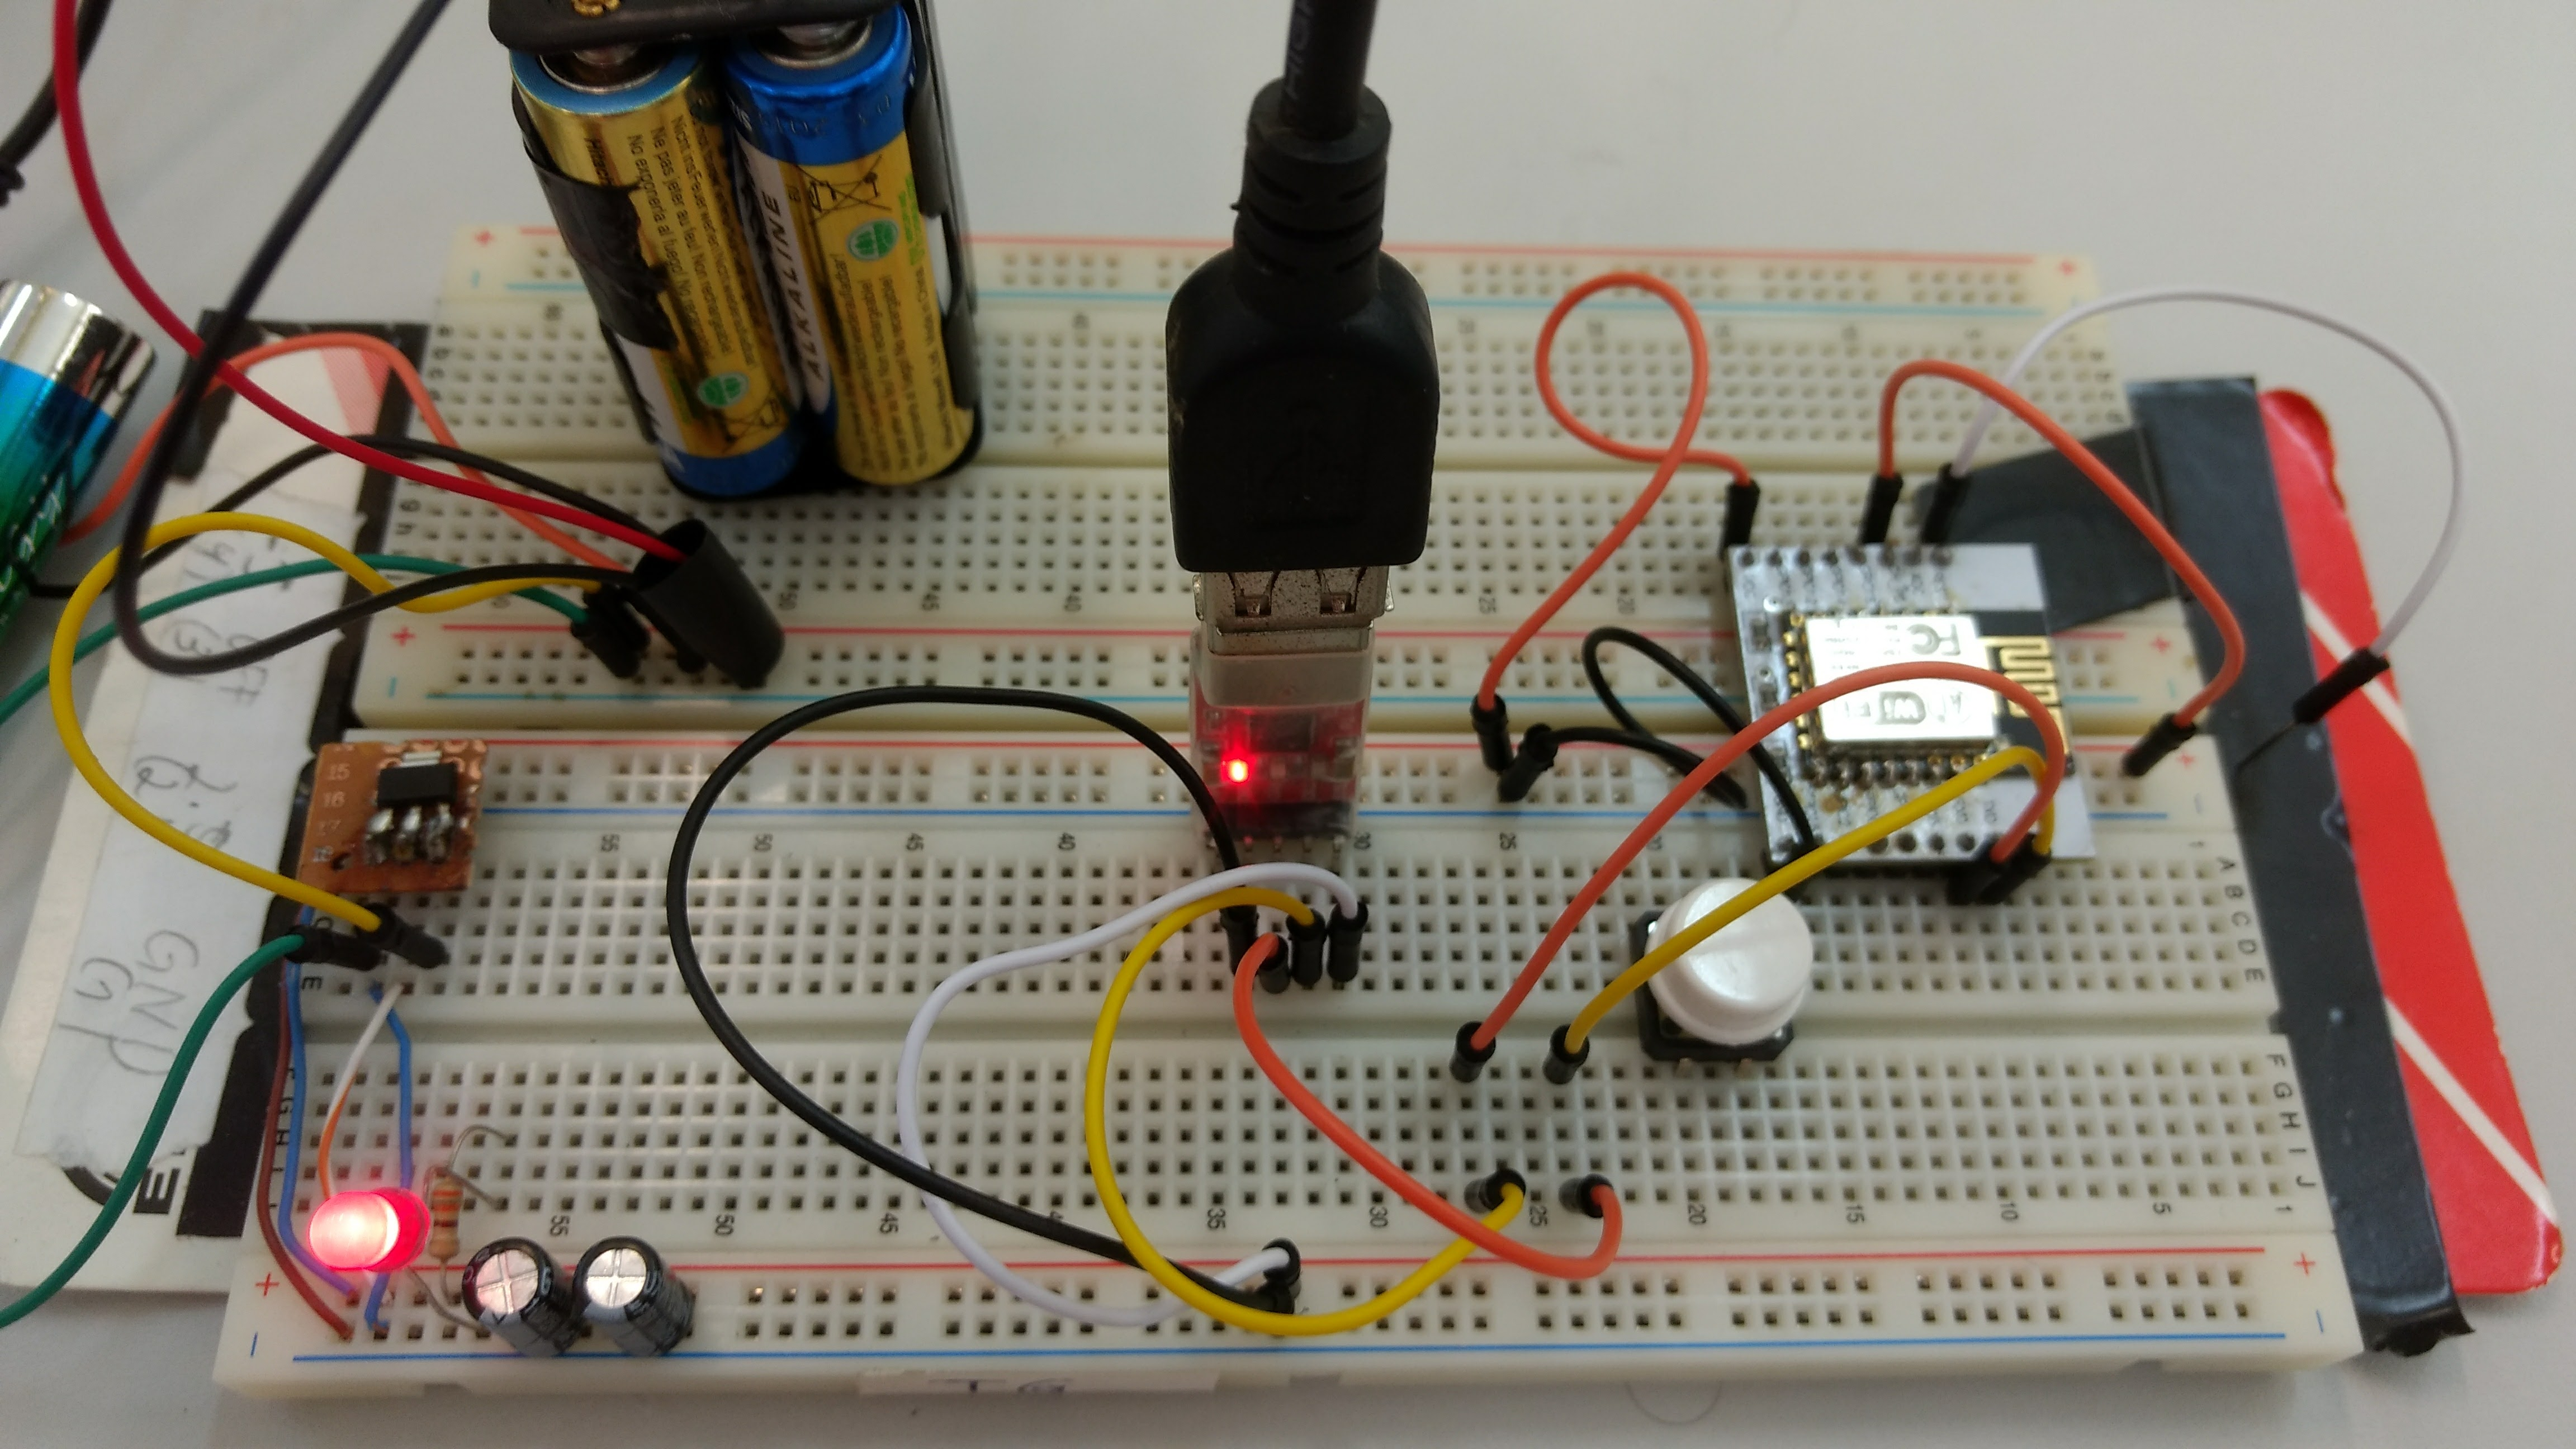
\includegraphics[width=1\textwidth]{040-plataformas/esp-dev/breadboard.jpg}
	\end{center}
	\legend{Fonte: Elaborada pelo autor}
\end{figure}

\emph{Carregadores}*

Todo código produzido em uma linguagem de programação é compilado por uma
ferramenta e, então, carrega-se os arquivos binários para o ESP8266 através da
serial, para que a execução do código seja iniciada. Na figura a seguir, é
apresentado um modelo de caminho desde o código até chegar no módulo ESP e,
também, a lista de carregadores usados.

\begin{figure}[htb]
	\caption{\label{fig:esp-toolchain}Modelo de processo de desenvolvimento e implantação com ESP8266}
	\begin{center}
		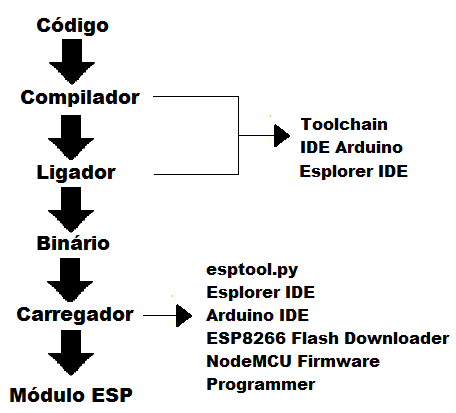
\includegraphics[width=1\textwidth]{040-plataformas/esp-dev/toolchain.png}
	\end{center}
	\legend{Fonte: Elaborada pelo autor}
\end{figure}


// mudar este paragrafo, simplificar

Todo código produzido é carregado para o módulo ESP através de seu barramento
serial. Alguns modelos, como o LoLin e D1 mini, já apresentam conversor serial
para micro USB. Para os que não possuem tal interface é necessário utilizar um
conversor serial - USB. As imagens a seguir demonstram como é o acesso de alguns
módulos utilizados. As GPIOs do ESP12F são acessadas somente através de placas
de circuito impresso, então uma foi adquirida para a programação do mesmo. Dos
conversores serial-USB adquiridos, o modelo CH340G não funcionou por não ter
driver compatível com o Windows 10, então a saída foi utilizar o modelo CP2102.


Os modos de programação descritos nas seções a seguir tem por objetivo acessar o
ponto da API de hardware do ESP8266 onde os pacotes destinados a outros
dispositivos são descartados,e habilitar o modo promíscuo.

Com a \emph{IDE Arduino}, a programação foi feita de primeiro modo através de um
\emph{firmware} genérico
chamado AT. Este é um conjunto de instruções enviados via serial para o módulo
ESP que permite configurá-lo. A \emph{IDE Arduino} e o \emph{Cool Term} possuem um emulador de
terminal serial que aceita os comandos AT e os envia direto para a serial.Além
disso, utilizou-se a linguagem C que foi compilada na \emph{IDE Arduino} e enviada ao
ESP.

Nenhuma dessas abordagens funcionou, pois nenhuma delas forneceu uma API que
funcionasse a baixo nível suficiente para atingir o modo promíscuo do ESP, que é
essencial para a descoberta de pacotes que trafegam entre dispositivos.

\begin{figure}[htb]
	\caption{\label{fig:esp-arduino}Código em C compilado e implantado em um ESP8266}
	\begin{center}
		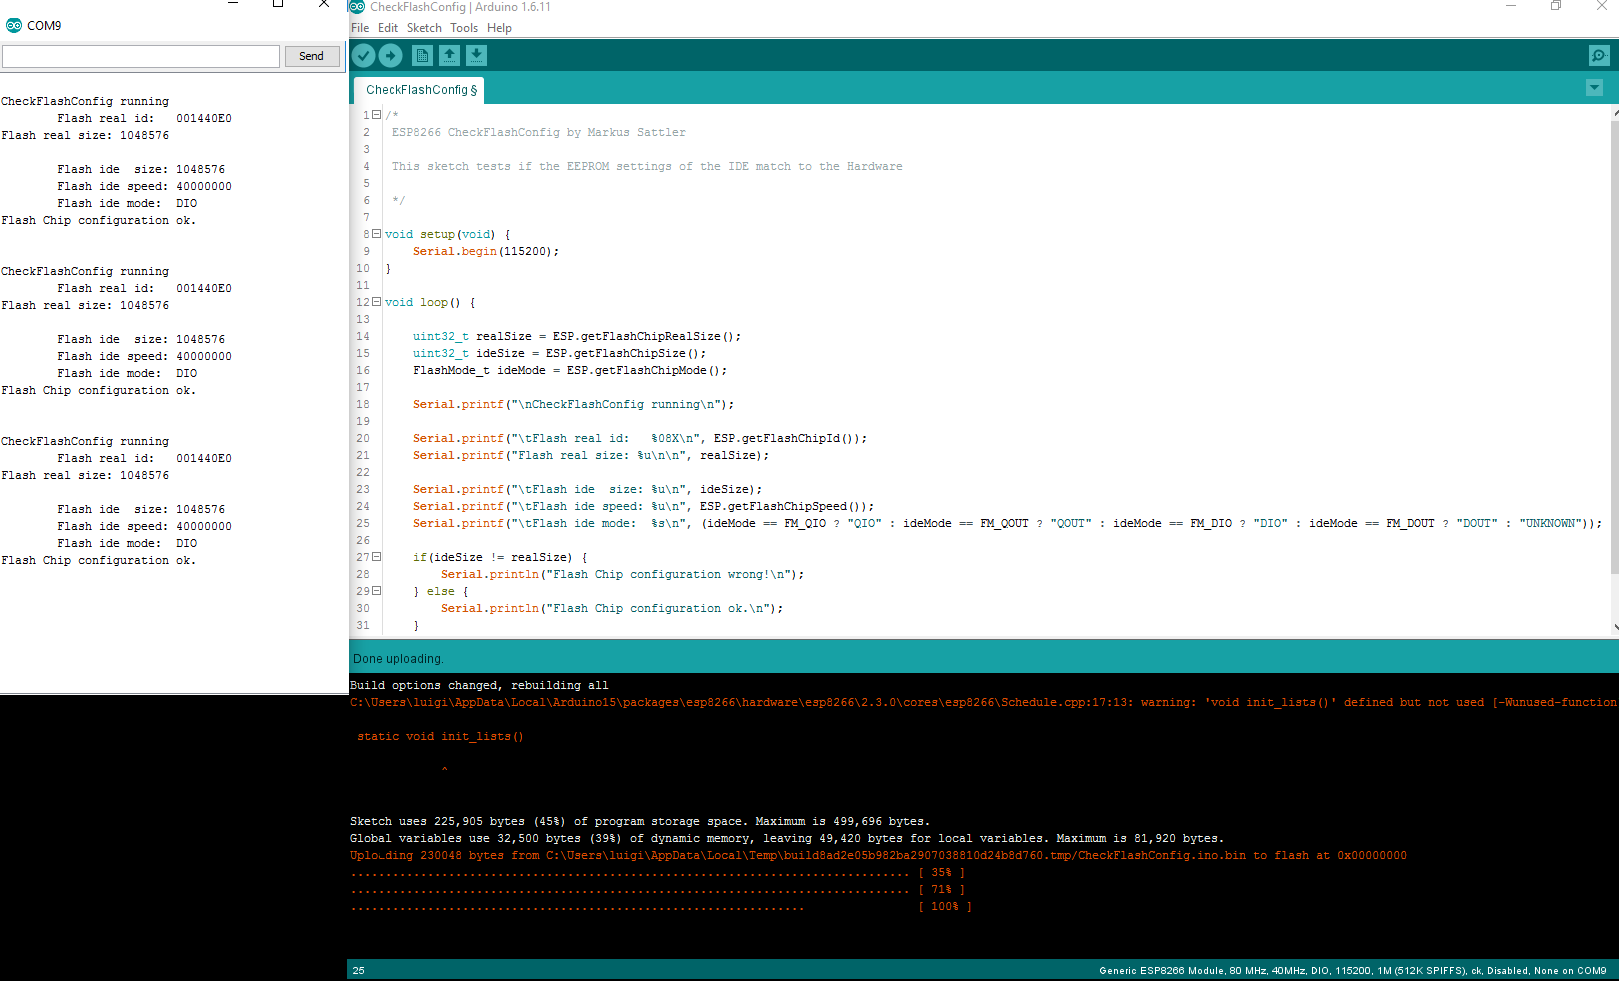
\includegraphics[width=1\textwidth]{040-plataformas/esp-dev/arduino-ide.png}
	\end{center}
	\legend{
	A esquerda comandos AT no emulador de serial da \emph{Arduino IDE}. //
	A direita editor da \emph{Arduino IDE} com código C //
	Abaixo em preto: processo de \emph{upload} do firmware escrito em C //
	Fonte: Elaborada pelo autor}
\end{figure}


*\emph{Toolchains}*

A segunda tentativa para a programação  dos módulos escolhidos foi feita através
de \emph{toolchains} (conjunto de ferramentas para desenvolvimento de software) da
empresa \emph{Espressif} e de um usuário do \emph{Github}, muito utilizado para projetos de
ESPs, Paulo Sokolovsky (\cite{pfalcon}). Ambas as \emph{toolchains} são \emph{SDKs} de código
aberto. Os \emph{scripts} foram feitos na linguagem C, compilados nessas SDKs e
transferidos para os módulos ESP. O maior problema dessas \emph{SDKs} foi a
configuração delas. Elas requisitavam de uma versão específica do Ubuntu que a
máquina utilizada para  fazer os códigos não suporta. Cogitou-se a possibilidade
de fazer máquinas virtuais, mas a máquina também não possui virtualização.

**Conclusão sobre o ESP**

Apesar do baixo custo e documentação da comunidade aberta, o ESP8266 não foi
adotado como sensor, pois não foi possível colocá-lo em modo prosmícuo,
essencial para detectar pacotes entre dispositivo e os pontos de acesso.

\section{Raspberry Pi}

**Especificações técnicas**

O Raspberry PI 3 Model B é um computador *single-board* (única placa) que tem o
tamanho próximo ao de um cartão de crédito. Foi desenvolvido pela Raspberry Pi
Foundation para promover o ensino da computação nas escolas. Este computador
possui:


\begin{alineas}
	\item Antena \emph{Wifi} embutida 802.11n;

	\item \emph{Bluetooth 4.1} e \emph{Bluetooth Low Energy} (BLE);

	\item 1 GB RAM;

	\item Processador Gráfico \emph{VideoCore IV 3D};

	\item ARM CPU de 1.2 GHz quad-core 64-bit.

	\item 4 portas USB;

	\item 40 pinos GPIOs;

	\item Porta HDMI;

	\item Porta \emph{Megabit Ethernet};

	\item Saída de aúdio e vídeo 3.5 mm;

	\item Interface para câmera (CSI) e monitor (DSI);

	\item Leitor para cartão \emph{micro SD};

\end{alineas}

\begin{figure}[htb]
	\caption{\label{fig:rpi-3}Raspiberry Pi 3 }
	\begin{center}
		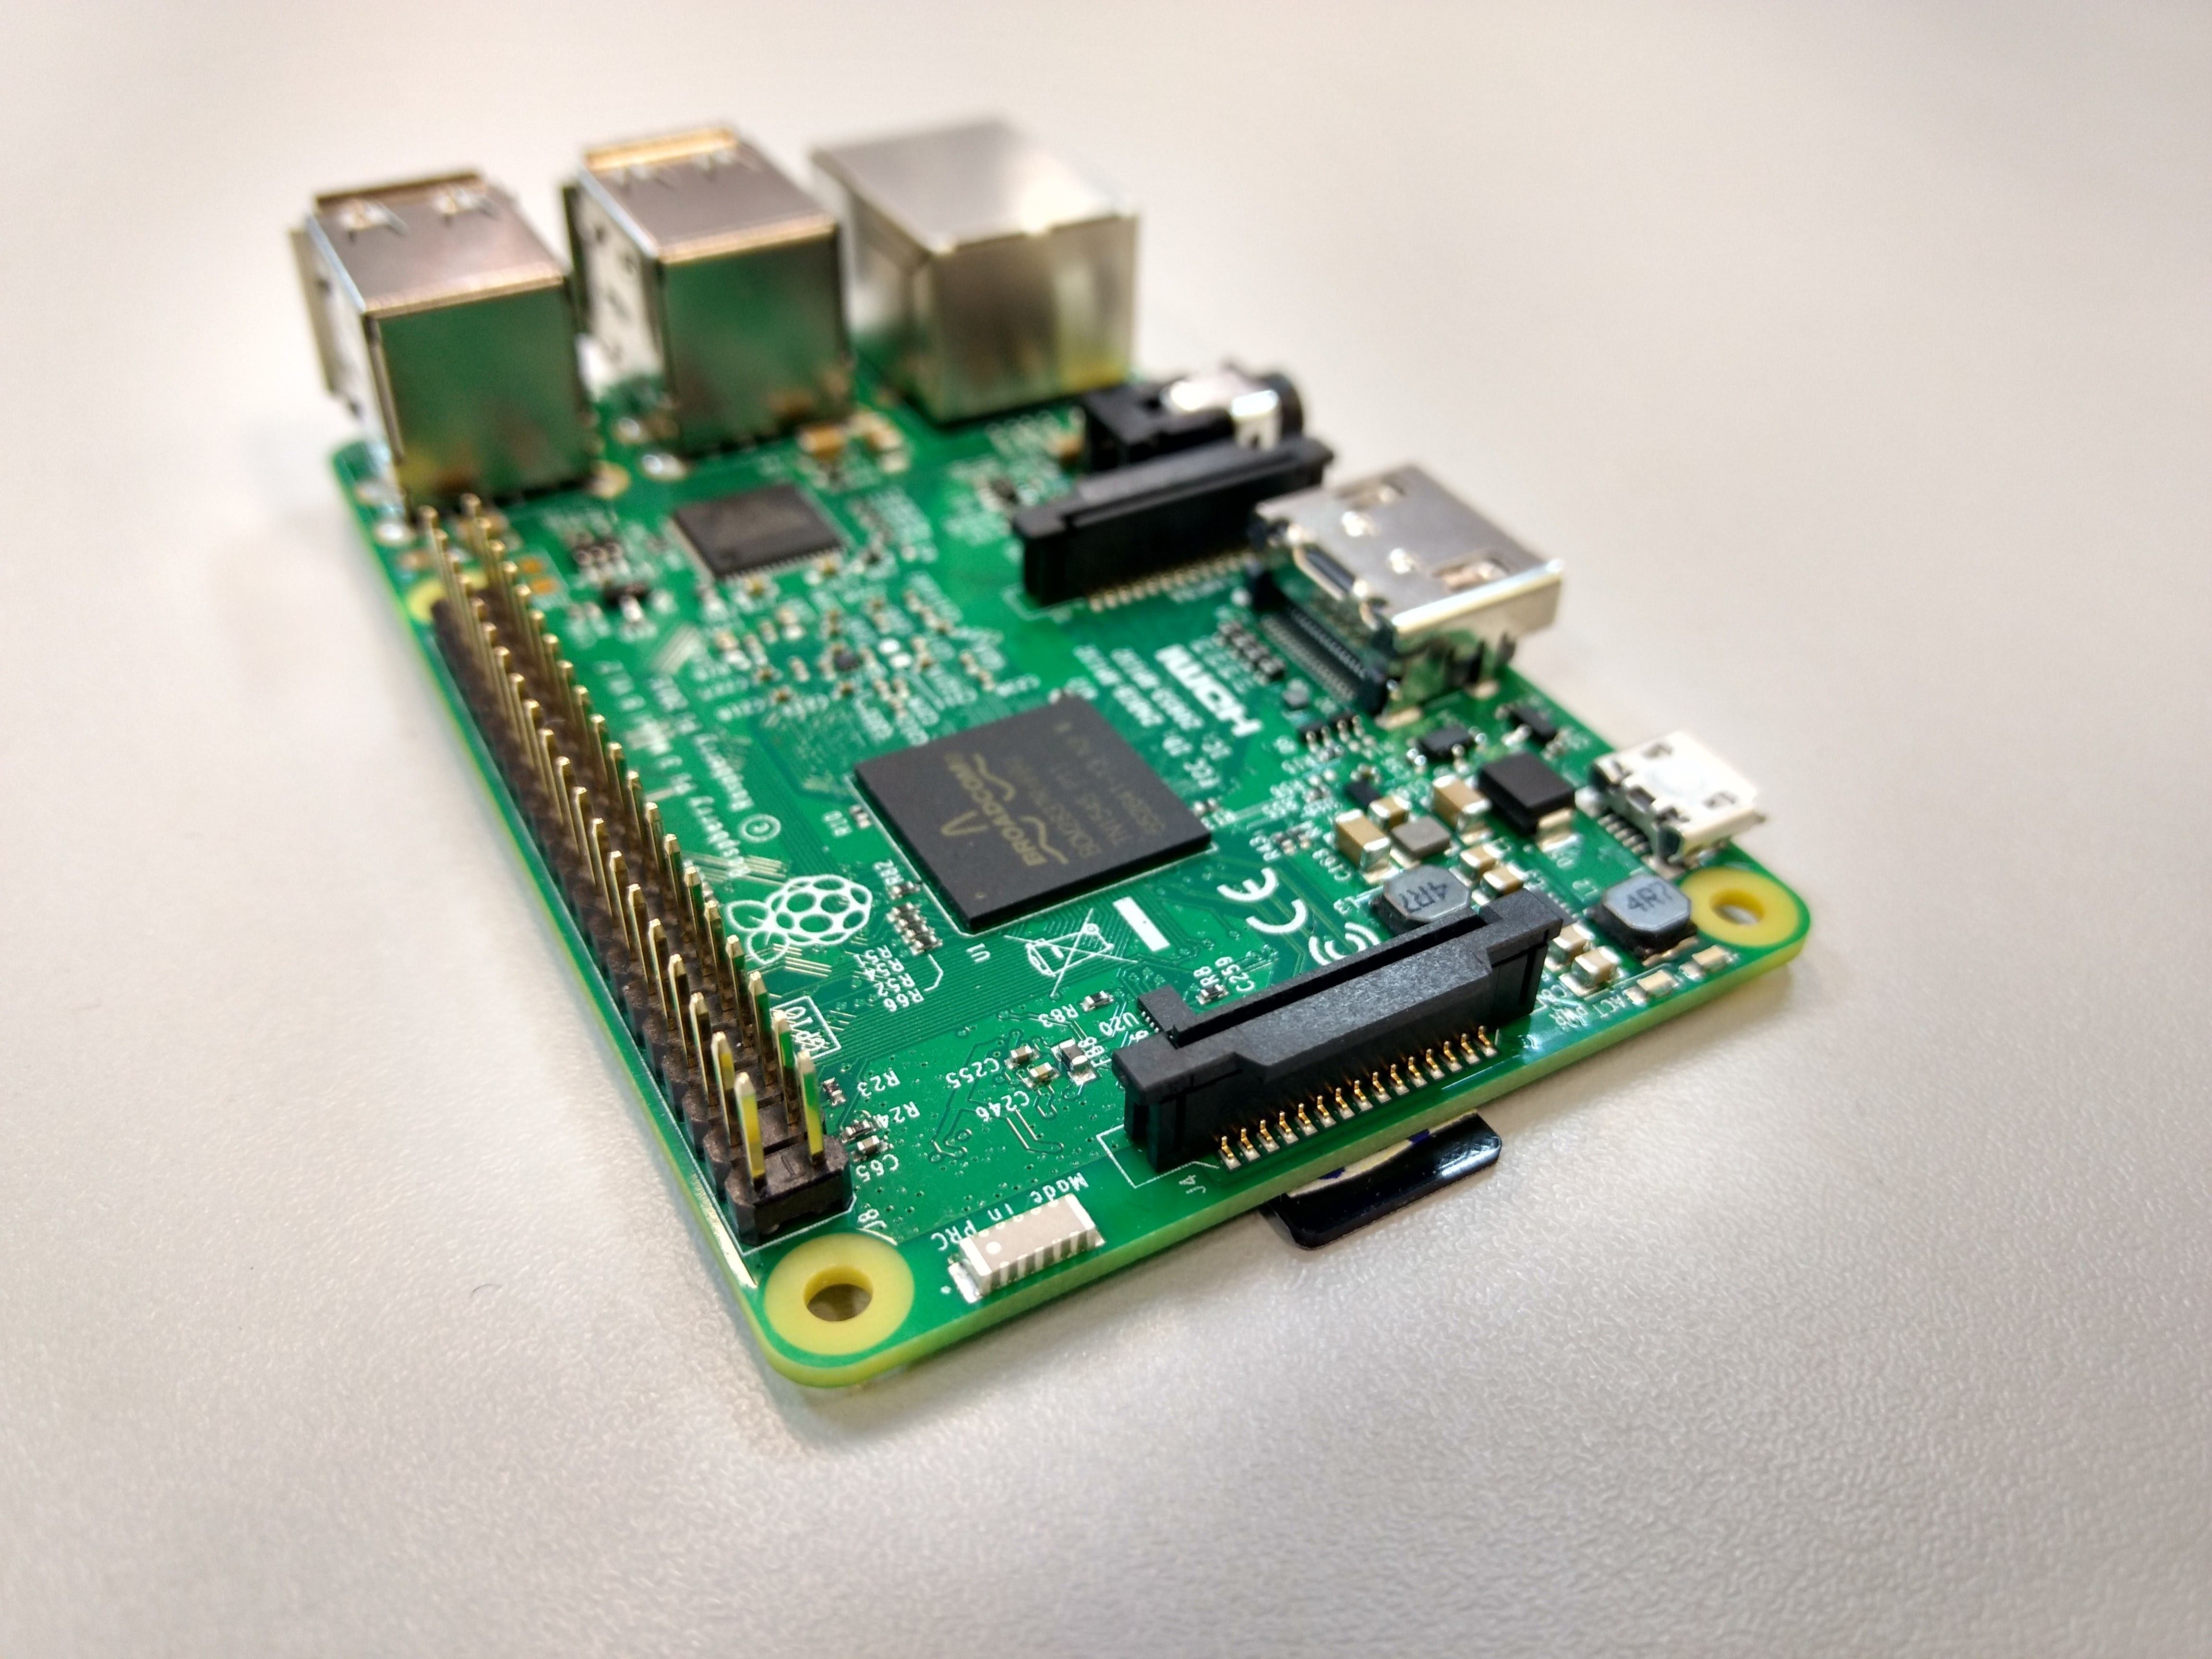
\includegraphics[width=1\textwidth]{040-plataformas/RPi-WiFi-dongles/rpi-onboard.jpg}
	\end{center}
	\legend{Fonte: Elaborada pelo autor}
\end{figure}

**Segunda tentativa**

Após da tentativa com o ESP8266, o Raspberry Pi foi escolhido como plataforma
para hospedar o sensor. Em média, no exterior, o RPi (Raspberry Pi) é vendido
por USD \$ 35,00 (Raspberry Foundation) e, no Brasil, por R\$ 250,00 (Mercado Livre).
Apesar de não ser tão barato como o ESP8266, ele possui recursos que facilitam a
programação e justificam seu preço.

A escolha deste dispositivo ocorreu principalmente devido a interface "amigável"
com usuário, comunidade *open source* e perfomance de processamento. Como o
Raspberry Pi "roda" um sistema operacional, o acesso a seus recursos e recursos
externos possui maior nível de abstração, bastando apenas alguns comandos para
acessá-los e estabelecer comunicação. Além de facilitar a programação destes
dispositivos por esse aspecto, com o sistema operacional IDEs externas podem ser
utilizadas.

Além deste recurso a nível de sistema, a comunidade e número de projetos "faça
você mesmo" é muito maior que a do ESP8266, devido a sua simplicidade em
conectar-se a um monitor e "sair" programando. Por ser um computador completo e,
dependendo do projeto, não é necessário mais nada além do RPi, pois ele possui
armazenamento, processamento e canal de comunicação (acesso à rede e portas
USB).

Outro aspecto é o processamento, como dito anteriormente, este computador possui
um poder de processamento para hospedar e processar inúmeras aplicações IoT.

**Alimentação**

O Raspberry é ligado por uma fonte de 2A, 5V e 10W através de uma entrada micro
USB. Para ligá-la, foi adquirido uma fonte USB tipo A para iPad, pois além de
poder desconectar o cabo da fonte, facilitando a manutenção, fornece a
quantidade exata de amperagem que o computador precisa. A primeira aquisição foi
de um carregador de \emph{smartphone} que não forneceu os amperes necessários.

Figura x.x - Carregador USB
![](carregador-ipad.jpg)

**Sistema Operacional**

O Raspberry Pi comporta sistemas operacionais que são carregados através no
micro cartão SD. Alguns exemplos de sistemas compatíveis: Archlinux, OpenELECE,
Raspbian, Risc, Pidora, Kali Linux, Windows 10 IoT, entre outros. Para este
trabalho, foi utilizado o Raspbian.

Figura X.X - Raspbian
![](raspbian.png)
Fonte: Elaborada pelo autor.

**Conclusão sobre Raspberry Pi**

O Raspberry foi adotado como o sensor para detectar os dispositivos. O modo
promíscuo conseguiu ser acessado através de adaptador/módulo USB Wifi. Mais
detalhes sobre a construção e adoção deste computador serão apresentados no
capítulo "Construção".

**Comparativo RPi X ESP8266**

Em comparação com o ESP8266, o Raspberry Pi compensou seu preço mais caro devido
a facilidade de programação e acesso aos seus recursos e integração e acesso a
recursos externos. Além disso, foi possível chegar ao modo promíscuo facilmente
através do Bash e do sistema operacional. A seguir, uma tabela comparando as
principais características do RPi e do módulo ESP12F.

Figura X.X - RPi x ESP12F
![](rpi-esp.png)
Fonte: Elaborada pelo autor.
